\chapter{Quality of Service}

\section{Network transmission}

\subsection{Network quality}

When the volume of traffic is greater than what can be transported across the network, devices queue, or hold, the packets in memory until resources become available to transmit them. If the number of packets to be queued continues to increase, the memory within the device fills up and packets are dropped.\\

Network congestion causes delay. Two types of delays are fixed and variable. A fixed delay is a specific amount of time a specific process takes, such as how long it takes to place a bit on the transmission media. A variable delay take an unspecified amount of time and is affected by factors such as how much traffic is being processed. Jitter is the variation in the delay of received packets.\\

A device implements QoS only when it is experiencing some type of congestion. Without any QoS mechanisms in place, packets are processed in the order in which they are received. When congestion occurs, network devices such as routers and switches can drop packets.\\

The \emph{playout delay buffer} must buffer these packets and then play them out in a steady stream. The \emph{digital signal processor (DSP)} interpolates what it thinks the audio should be and no problem is audible to the user. 

\subsection{Traffic characteristics}

\subsubsection{Voice}

Voice traffic is predictable and smooth, as shown in the figure. However, voice is very sensitive to delays and dropped packets; there is no reason to re-transmit voice if packets are lost. Therefore, voice packets must receive a higher priority than other types of traffic.\\

Latency should be no more than 150 milliseconds (ms). Jitter should be no more than 30 ms, and voice packet loss should be no more than 1\%. Voice traffic requires at least 30 Kbps of bandwidth.

\subsubsection{Video}

Video traffic tends to be unpredictable, inconsistent, and bursty compared to voice traffic. Compared to voice, video is less resilient to loss and has a higher volume of data per packet.\\

Latency should be no more than 400 milliseconds (ms). Jitter should be no more than 50 ms, and video packet loss should be no more than 1\%. Video traffic requires at least 384 Kbps of bandwidth.

\subsubsection{Data}

Data traffic is relatively insensitive to drops and delays compared to voice and video. The two main factors a network administrator needs to ask about the flow of data traffic are the following: Does the data come from an interactive application? Is the data mission critical?

\section{Queueing algorithms}
Queuing is a congestion management tool that can buffer, prioritize, and, if required, reorder packets before being transmitted to the destination.

\subsection{WFQ}

WFQ (Weighted Fair Queuing) is an automated scheduling method that provides fair bandwidth allocation to all network traffic. \\

WFQ applies priority, or weights, to identified traffic and classifies it into conversations or flows, as shown in the figure \ref{WFQ}. WFQ then determines how much bandwidth each flow is allowed relative to other flows. WFQ classifies traffic into different flows based on packet header addressing (IP addresses, MAC addresses, port numbers, protocol, and ToS value).\\

\begin{figure}[hbtp]
\caption{WFQ example}\label{WFQ}
\centering
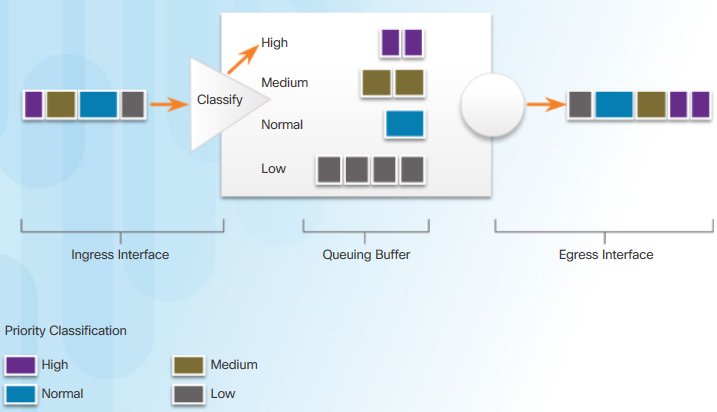
\includegraphics[ width=0.8\textwidth ]{pictures/WFQ.PNG}
\end{figure}

WFQ has limitations. It is not supported with tunneling and encryption. It does not offer the degree of precision control over bandwidth allocation that CBWFQ offers.

\subsection{CBWFQ}

Class-Based Weighted Fair Queuing (CBWFQ) extends the standard WFQ functionality to provide support for user-defined traffic classes. For CBWFQ, you define traffic classes based on match criteria including protocols, access control lists (ACLs), and input interfaces. A FIFO queue is reserved for each class, and traffic belonging to a class is directed to the queue for that class, as shown in the figure.\\

To characterize a class, you assign it bandwidth, weight, and queue limit. After a queue has reached its configured queue limit, adding more packets to the class causes tail drop. Tail drop means a router simply discards any packet that arrives at the tail end of a queue that has completely used up its packet-holding resources.\\

\subsection{LLQ}

The Low Latency Queuing (LLQ) feature brings strict priority queuing (PQ) to CBWFQ. Strict PQ allows delay-sensitive data such as voice to be sent before packets in other queues.\\

Without LLQ, CBWFQ services fairly based on weight; no class of packets may be granted strict priority. This scheme poses problems for voice traffic that is largely intolerant of delay, especially variation in delay. With LLQ, delay-sensitive data such as voice is sent first (before packets in other queues).

\section{QoS models}
The three models for implementing QoS are: Best-effort model, Integrated services (IntServ), Differentiated services (DiffServ). QoS is really implemented in a network using either IntServ or DiffServ.

\subsection{Best effort}

The best-effort model (meaning no QoS) treats all network packets in the same way, so an emergency voice message is treated the same way a digital photograph attached to an email is treated. The table \ref{BestEffort} in the figure lists the benefits and drawbacks of the best effort model. 

\begin{table}[hbtp]
\centering
\caption{Pros and Cons of Best-effort}\label{BestEffort}
\begin{tabular}{ll}
\toprule
\head{Benefits} & \head{Drawbacks} \\ 
\midrule 
Most scalable & No guarantees of delivery \\  
Scalability is limited by bandwidth & Packets can arrive in any order \\ 
No special QoS mechanism required & No packets have preferential treatment \\ 
Easy to deploy & Critical data is treated the same as casual one \\ 
\bottomrule
\end{tabular}
\end{table} 

\subsection{Integrated services}

Integrated Services (IntServ) is a multiple-service model that can accommodate multiple QoS requirements.\\

It uses resource reservation and admission-control mechanisms as building blocks to establish and maintain QoS. Each individual communication must explicitly specify its traffic descriptor and requested resources to the network (Figure \ref{IntServ}). The edge router performs admission control to ensure that available resources are sufficient in the network.\\

\begin{figure}[hbtp]
\caption{Simple IntServ example}\label{IntServ1}
\centering
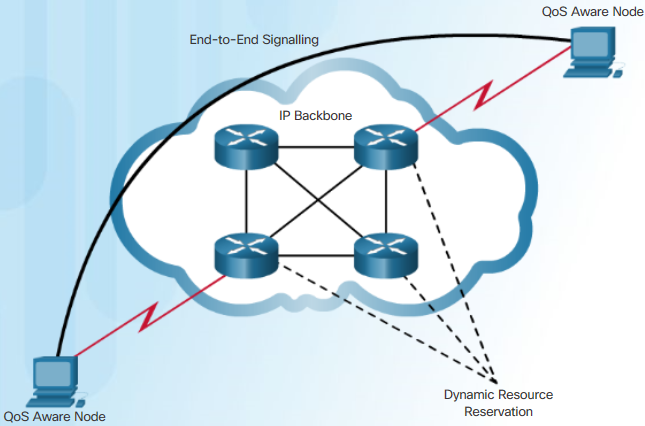
\includegraphics[scale=0.7]{pictures/IntServ.PNG}
\end{figure}


IntServ uses the Resource Reservation Protocol (RSVP) to signal the QoS needs of an application’s traffic along devices in the end-to-end path through the network. The table \ref{IntServ2} lists the benefits and drawbacks of the IntServ model.

\begin{table}[hbtp]
\centering
\caption{Pros and Cons of IntServ}\label{IntServ2}
\begin{tabular}{ll}
\toprule
\head{Benefits} & \head{Drawbacks} \\ 
\midrule 
Explicit end-to-end resource admission control & Resource intensive \\  
Per-request policy admission control & Not scalable \\ 
Signaling of dynamic port numbers &  \\ 
\bottomrule
\end{tabular}
\end{table} 

\subsection{Differentiated services}

The DiffServ design overcomes the limitations of both the best-effort and IntServ models. Unlike IntServ and hard QoS in which the end-hosts signal their QoS needs to the network, DiffServ does not use signaling. It works on the provisioned-QoS model, where network elements are set up to service multiple classes of traffic each with varying QoS requirements (Figure \ref{DiffServ1}).\\

\begin{figure}[hbtp]
\caption{Simple DiffServ example}\label{DiffServ1}
\centering
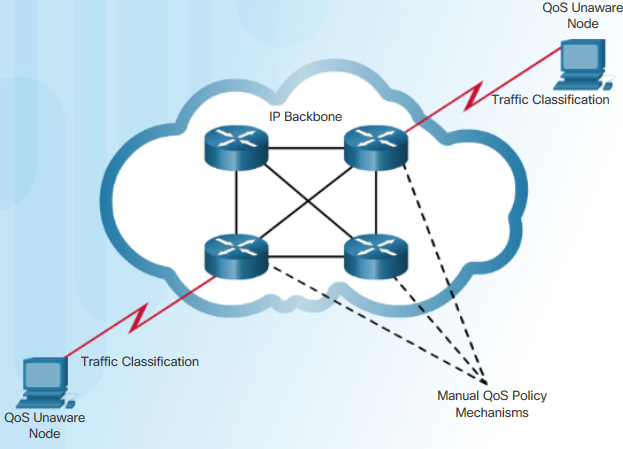
\includegraphics[scale=0.7]{pictures/DiffServ.PNG}
\end{figure}


As a host forwards traffic to a router, the router classifies the flows into aggregates (classes) and provides the appropriate QoS policy for the classes. DiffServ enforces and applies QoS mechanisms on a hop-by-hop basis, uniformly applying global meaning to each traffic class to provide both flexibility and scalability.\\

Table \ref{DiffServ2} lists the benefits and drawbacks of the DiffServ model.

\begin{table}[hbtp]
\centering
\caption{Pros and Cons of DiffServ}\label{DiffServ2}
\begin{tabular}{ll}
\toprule
\head{Benefits} & \head{Drawbacks} \\ 
\midrule 
Highly scalable & No absolute guarantee of delivery \\  
Many different levels of quality & Requires complex mechanisms \\ 
\bottomrule
\end{tabular}
\end{table} 

\section{QoS implementation}

\subsection{Classification and Marking}

Before a packet can have a QoS policy applied to it, the packet has to be classified. Classification and marking allows us to identify or mark types of packets. Marking means that we are adding a value to the packet header. Devices receiving the packet look at this field to see if it matches a defined policy.\\

Traffic should be classified and marked as close to its source as technically and administratively feasible. This defines the trust boundary.\\

Trusted endpoints have the capabilities and intelligence to mark application traffic to the appropriate Layer 2 CoS and/or Layer 3 DSCP values. Examples of trusted endpoints include IP phones, wireless access points, videoconferencing gateways and systems, IP conferencing stations, and more.

\subsubsection{Marking at Layer 2}

802.1Q is the IEEE standard that supports VLAN tagging at layer 2 on Ethernet networks. The 802.1Q standard also includes the QoS prioritization scheme known as IEEE 802.1p. The 802.1p standard uses the first three bits in the Tag Control Information (TCI) field (Figure \ref{CoS}). Known as the Priority (PRI) field, this 3-bit field identifies the Class of Service (CoS) markings.\\

\begin{figure}[hbtp]
\caption{Ethernet Class of Service values}\label{CoS}
\centering
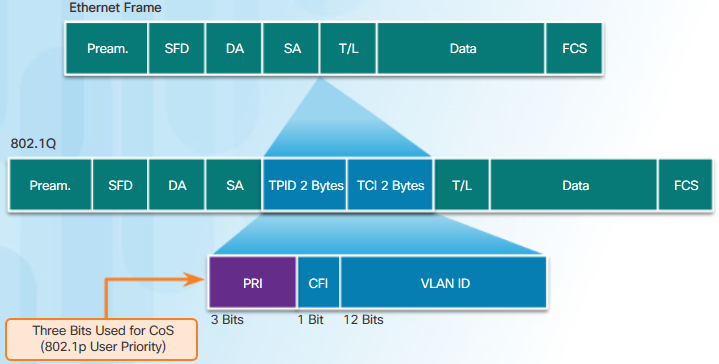
\includegraphics[ width=0.8\textwidth ]{pictures/CoS.PNG}
\end{figure}

\subsubsection{Marking at Layer 3}

Both IPv4 and IPv6 support an 8-bit field for marking, the Type of Service (ToS) field for IPv4 and the Traffic Class field for IPv6. Figure \ref{ToS} displays the contents of the 8-bit field. The field has 6-bits allocated for QoS, called the \textbf{DiffServ} Code Point (DSCP) field. The remaining two IP Extended Congestion Notification (ECN) bits can be used by ECN-aware routers to mark packets instead of dropping them. The ECN marking informs downstream routers that there is congestion in the packet flow. \\

\begin{figure}[hbtp]
\caption{Type of Service/Traffic Class Field}\label{ToS}
\centering
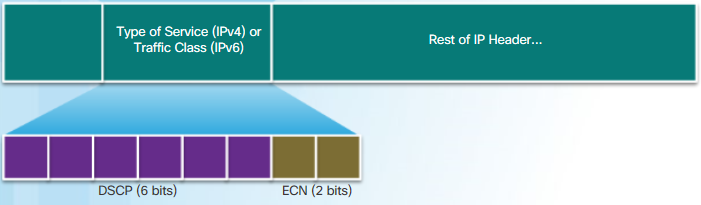
\includegraphics[ width=0.8\textwidth ]{pictures/ToS.PNG}
\end{figure}

The DSCP values are organized into three categories: 
\begin{description}
\item[Best-Effort (BE)]When a router experiences congestion, these packets will be dropped. No QoS plan is implemented.
\item[Expedited Forwarding (EF)]DSCP decimal value is 46 (binary 101110). At Layer 3, Cisco recommends that EF only be used to mark voice packets.
\item[Assured Forwarding (AF)] use the 5 most significant DSCP bits to indicate queues and drop preference. As shown in Figure \ref{DSCP}, the first 3 most significant bits are used to designate the class. The 4th and 5th most significant bits are used to designate the drop preference. The 6th most significant bit is set to zero. The AFxy formula shows how the AF values are calculated. For example, AF32 belongs to class 3 (binary 011) and has a medium drop preference (binary 10).
\end{description}

\begin{figure}[hbtp]
\caption{Assured forwarding values}\label{DSCP}
\centering
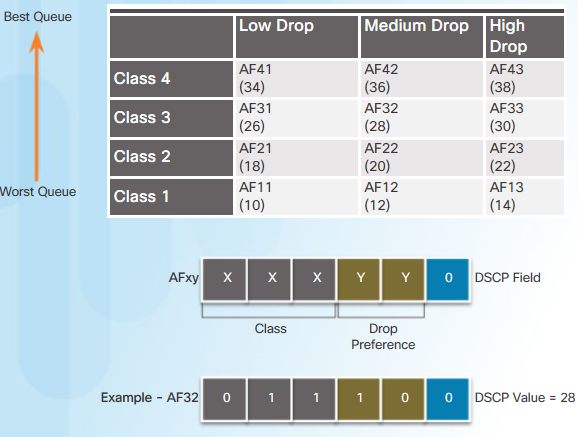
\includegraphics[ scale=0.7 ]{pictures/DSCP.PNG}
\end{figure}

\subsection{Congestion Avoidance}

Congestion avoidance tools are simpler than Congestion management. These tools can monitor the average depth of the queue, as represented in the figure. When the queue is below the minimum threshold, there are no drops. As the queue fills up to the maximum threshold, a small percentage of packets are dropped. When the maximum threshold is passed, all packets are dropped.\\

Cisco IOS QoS includes weighted random early detection (WRED) as a possible congestion avoidance solution. Using WRED helps avoid tail drops and maximizes network use and TCP-based application performance. In case of UDP-based traffic, methods such as queuing and compression techniques help to reduce and even prevent UDP packet loss.

\subsection{Shaping and Policing}

Traffic shaping and traffic policing are two mechanisms provided by Cisco IOS QoS software to prevent congestion. 

\subsubsection{Traffic shaping}

Traffic shaping retains excess packets in a queue and then schedules the excess for later transmission over increments of time. The result of traffic shaping is a smoothed packet output rate, as shown in Figure \ref{Spacing}.\\

\begin{figure}[hbtp]
\caption{Spacing traffic example}\label{Spacing}
\centering
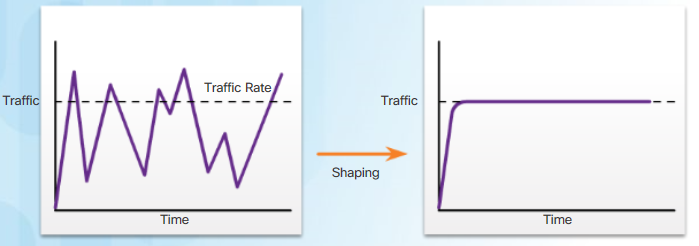
\includegraphics[scale=0.7]{pictures/Spacing.PNG}
\end{figure}

Ensure that you have sufficient memory when enabling shaping. In addition, shaping requires a scheduling function (CBFWQ, LLQ) for later transmission of any delayed packets.

\subsubsection{Traffic policing}

Shaping is an outbound concept; packets going out an interface get queued and can be shaped. In contrast, policing is applied to inbound traffic on an interface. When the traffic rate reaches the configured maximum rate, excess traffic is dropped (or remarked). See also Figure \ref{policing}.\\

\begin{figure}[hbtp]
\caption{Spacing traffic example}\label{policing}
\centering
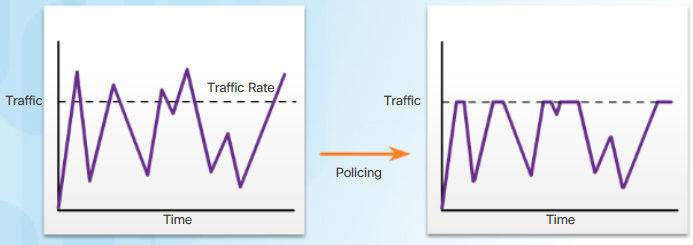
\includegraphics[ scale=0.7 ]{pictures/policing.PNG}
\end{figure}

Ensure that you have sufficient memory when enabling shaping. In addition, shaping requires a scheduling function (CBFWQ, LLQ) for later transmission of any delayed packets.
